\chapter{Introduction}
    %\addcontentsline{toc}{chapter}{\protect\numberline{}Introduction}
    
     % Might be useful: http://www.emerson.emory.edu/services/latex/latex_162.html

\section{General context}

In the last century, the field of aeronautics has experimented huge advances since airplanes became a fundamental tool during the World War I. The advances in military aviation during this period were followed by the apparition of the first commercial airplanes and the birth of  

The steep growth of aviation and gas turbines has also led to an 

During the last century, aviation has not stopped growing since it became a fundamental 

Since the beginning of aviation at the end


ACARE target for 2020, vs ACARE target for 


\begin{figure}[h!]
	\centering
	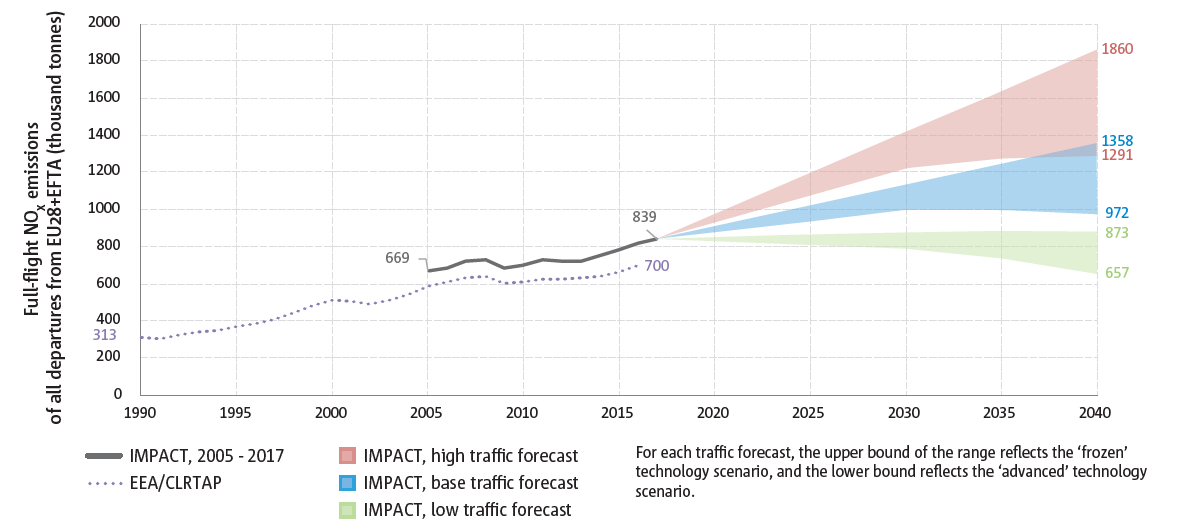
\includegraphics[scale=0.5]{./part0_intro/NOx_emissions_forecast_report2019}
	\caption{Atomization breakup regimes \citepColor[herrmann_modeling_2003]}
	\label{fig:atomization_regimes_herrmann}
\end{figure}


%\section{Motivation}

%\section{Lean-premixed systems for pollutant reduction}
\section{Lean combustion in gas turbines}

With the objective of reducing pollutant emissions, engine manufacturers have 

Show graph NOx formation versus temperature.



\section{Fuel injection technology}

\begin{figure}[h!]
	\centering
	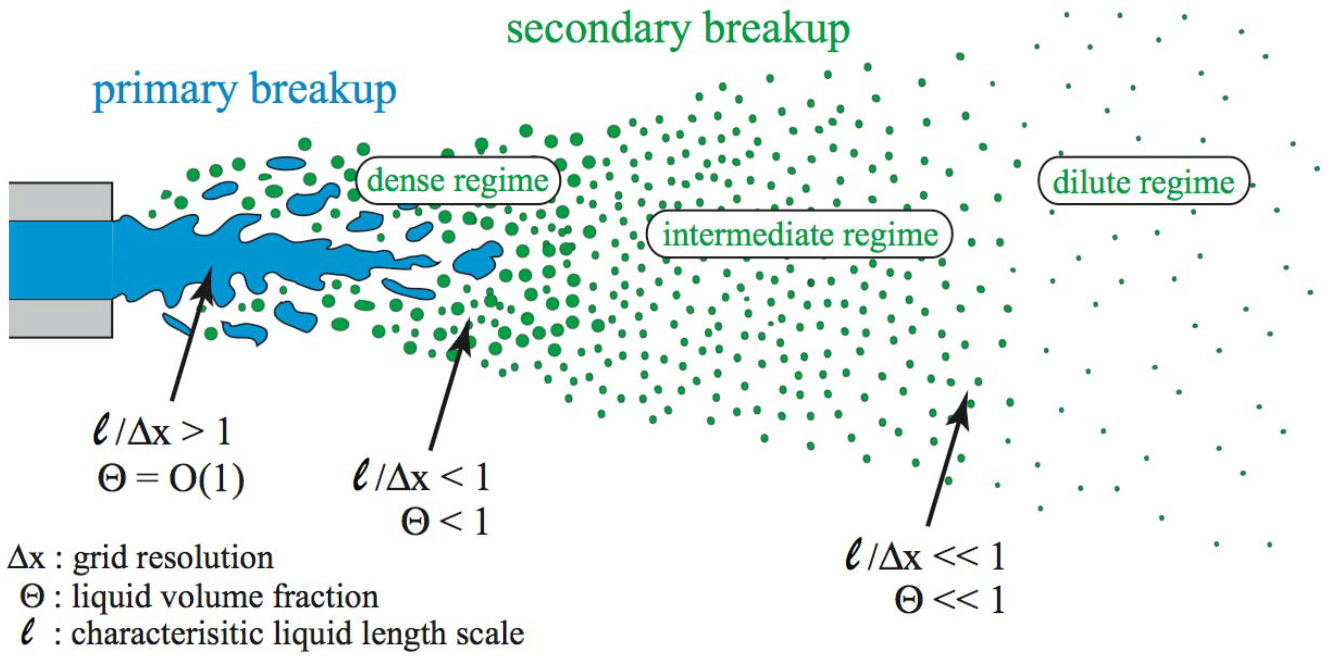
\includegraphics[scale=0.5]{./part0_intro/atomization-regimes-scheme}
	\caption{Atomization breakup regimes \citepColor[herrmann_modeling_2003]}
	\label{fig:atomization_regimes_herrmann}
\end{figure}

\subsection*{Atomization process}

Explain two-phase flows phenomenology (injection + atomization) here. 

Explain airblast, hollow-cone, jicf.

\section{Objective and thesis outline}
    %\addcontentsline{toc}{section}{\protect\numberline{}Manuscript organisation}

